\documentclass[]{beamer}


\usepackage{amsmath}
\usepackage{amssymb}
\usepackage{graphicx}
\usepackage{subfiles}
\usepackage{framed}
\usepackage{enumerate}

%opening
\title{}
\author{}

\begin{document}

\section*{Survival Analysis}
	
\begin{frame}	
\noindent{Introduction to Survival Analysis}

Survival analysis models factors that influence the time to an event. Ordinary least squares regression methods fall short because the time to event is typically not normally distributed, and the model cannot handle censoring, very common in survival data, without modification. 

\end{frame}
	
	\section{What is Survival Analysis?}
	\begin{frame}
		
		%Survival Analysis part 1: 
		\noindent \textbf{What is Survival Analysis?}
		
		\begin{itemize}
			\item Survival analysis is generally defined as a set of methods for analyzing data where the outcome variable is the time until the occurrence of an event of interest. The event can be death, occurrence of a disease, marriage, divorce, etc.
			
			\item	Survival analysis is long established within actuarial science and medical research but seems infrequently used in general data science projects. 
			\item Time-to-event analyses are very widely applicable to all sorts of real-world behaviours - not just studies of lifespan in actuarial or medical science.
		\end{itemize}
		
		
	\end{frame}
	%=================================%
	\begin{frame}
		\frametitle{Survival Analysis}
		In this series of blogposts:	
		\begin{itemize}
			\item We'll introduce survival analysis as a vital technique in any statisticians toolkit
			
			\item We'll demonstrate a general approach to undertaking a data science project: accessing, cleaning and storing data, and using a range of open-source analytical tools that enable rapid iteration, data exploration, modelling and visualisation
			
			\item We'll use a real-world dataset and seek to both match and improve upon some existing analysis already undertaken and released by a third-party.
		\end{itemize}	
		
	\end{frame}
	%=================================%
	\begin{frame}
		\frametitle{Survival Analysis}
		By the end you should have a better understanding of the theory, some tools and techniques, and hopefully gain some ideas about how survival analysis can be applied to all manner of event-based processes that are often crucial to business operations.
		
		So firstly...
	\end{frame}
	%=================================%
	\begin{frame}
		\frametitle{Survival Analysis}
		What is Survival Analysis?
		Wikipedia defines survival analysis as:
		
		a branch of statistics that deals with analysis of time duration until one or more events happen, such as death in biological organisms and failure in mechanical systems.
	\end{frame}
	%=================================%
	\begin{frame}
		\frametitle{Survival Analysis}
		\large
		\noindent \textbf{Actuarial Application}
		\begin{itemize}
			\item We might, for example, expect an actuary to try to predict what proportion of the general population will survive past a certain age. 
			\item The actuary might want to furthermore know the rate of change of survival with time (the hazard function), and the characteristics of individuals which most influence their survival.
		\end{itemize}
		
		
	\end{frame}
	%=================================%
	\begin{frame}
		\frametitle{Survival Analysis}
		More generally, we can use survival analysis to model the expected time-to-event for a wide variety of situations:
		\begin{itemize}
			\item \textbf{User shopping behaviour} e.g. the elapsed time between a user subscribing to an online shopping service and ordering their first product
			\item \textbf{Crop yields and harvesting} e.g. the duration between seeding a field and the majority of the crops being ready for harvest
			\item \textbf{Radioactive halflife} e.g. the time until half the atoms in a luminous blob2 of tritium have decayed into hydrogen and helium-3
			\item \textbf{Hardware failure rates} e.g. the expected lifetime for a piece of machinery before component failure.
			\item \textbf{Customer subscription persistence} e.g. the expected time for a customer to remain subscribed to a cellphone service before churning
			
		\end{itemize}
	\end{frame}
	%=================================%
	\begin{frame}
		\frametitle{Survival Analysis}
		Illustrating the basics
		\begin{itemize}
			\item Imagine we have a fleet of haulage trucks and we're particularly interested in the elapsed time between purchase and first maintenance event (aka repairs aka servicing). We could use this analysis to:
			
			\item Identify which manufacturers and models of trucks require the least repair and favour buying those again in future
			
			\item Identify contributing factors leading to trucks needing earlier repairs and try to mitigate
			
			\item Anticipate likely spikes of activity for fleet repair during the year and ensure funds are available in advance
			
		\end{itemize}
		
	\end{frame}
	\section{Sketching a survival curve}
	%=================================%
	\begin{frame}
		\frametitle{Survival Analysis}
		Sketching a survival curve
		% Illustration of survival curve and half-life
		We observe:
		
		The relative duration of our study is measured from time of purchase until the end of the second year (24 months). This is a relative time and may begin at a different time for each truck
		
		The survival function is a measure of how many trucks are serviced at each point in time. It drops quickly and then flattens out; it crosses the 50\% line at 10 months, meaning that by 10 months we can expect 50\% of all the trucks in the fleet to have had their first service.
		
		About 36\% of trucks remain unserviced at the end of the first 24 months; conversely, about 64\% will have a service event during their first 24 months
	\end{frame}
	%=================================%
	\section{Two fundamental measurements}
	\begin{frame}
		\frametitle{Survival Analysis}
		\noindent \textbf{Fundamental Measurements: The survival function S(t)} \\
		
		The survival function, $S(t)$, of an individual is the probability that they survive until at least time tt.
		
		\[S(t)=Pr(T>t)\]
		where $t$ is a time of interest and $T$ is the time of event.
		
		The survival curve is non-increasing (the event may not reoccur for an individual) and is limited within [0,1]. Note that the event might not happen within our period of study and we call this right-censoring. This happens in the above example where for 36\% of trucks, all we know is that their first service happens some time after 24 months.
	\end{frame}
	%=================================%
	\begin{frame}
		\frametitle{Survival Analysis}
		\noindent \textbf{The hazard function $\lambda(t)$} % λ(t)
		The hazard function $\lambda(t)$ is a related measure, telling us the probability that the event TT occurs in the next instant $t+ \delta t$, given that the individual has reached timestep $t$:
		
		\[\lambda(t)=\lim _{\delta_t \rightarrow 0} Pr(t \leq T<t+\delta_t | T>t) \delta_t\]
		
		With some maths we can work back to the Survival function:
		
		\[S(t)=exp(−\int \lambda(u)du)\]
		
		The hazard function $\lambda(t)$ is non-parametric, so we can fit a pattern of events that is not necessarily monotonic.
		
	\end{frame}
	%=================================%
	\begin{frame}
		\frametitle{Survival Analysis}
		
		\noindent \textbf{Other measurements and considerations}\\
		
		\begin{itemize}
			\item The cumulative hazard function is an alternative representation of the time-to-event behaviour is the cumulative hazard function $\Lambda(t)$, which is essentially the summing of the hazard function over time, and is used by some models for its greater stability. We can show:
			
			\[ \Lambda(t)=\int_0^t \lambda(u)du = - logS(t)\]
			
			\item The simple relation of $\Lambda(t)$ to the survival function $S(t)$ is a nice property, exploited in particular by the Cox Proportional Hazards and Aalen Additive models, which we'll demonstrate later.
		\end{itemize}
		
	\end{frame}
	%=================================%
	\begin{frame}
		\frametitle{Survival Analysis}
		Stating it slightly differently, we can relate the attributes of the individuals to their survival curve:
		
		% S(t)=−e∑Λi(t)
		
		This powerful approach is known as \textbf{\textit{Survival Regression}}. In the trucks example, we might want to know the relative impact of engine size, hours of service, geographical regions driven etc upon the time from first purchase to first service.
	\end{frame}
	%=================================%
	\section{The Half Life}
	\begin{frame}
		\frametitle{Survival Analysis}
		\noindent \textbf{The half-life}
		\begin{itemize}
			\item We saw the half-life of truck repair illustrated above (the orange arrows). 
			\item Most people are familiar with this measure and it's exactly as it says on the tin:
			
			select a group of individuals - our fleet of trucks - and measure how long it takes for the event of interest to occur.
			once the event of interest - the first service repair - occurs for half of the population, that period is aka the half-life.
			note that we can't state exactly which truck or exactly when, just work on the aggregate values.
			\item There's nothing particularly special about the half-life, and we might be interested in the time taken for e.g. 25\% of the trucks to come in for first service, or 75\% or 90\% etc.
		\end{itemize}
		
	\end{frame}


	\section{Nelson-Aalen Model}
	%=================================%
	\begin{frame}
		\frametitle{Survival Analysis}
		\textbf{Nelson-Aalen Model}
		\begin{itemize}
			\item A close alternative method is the Nelson-Aalen model, which estimates the cumulative hazard function $\Lambda(t)=-\log S(t)$ and is more stable since it has a summation form:
			%	
			%	
			%	% Λ^(t)=∑ti≤tdini
			%	
			where again, $d$ and $n$ are respectively the count of 'death' events and individuals at risk at timestep $i$.
			\item 
			The estimator is given by
			
			\[ {\displaystyle {\tilde {H}}(t)=\sum _{t_{i}\leq t}{\frac {d_{i}}{n_{i}}},}  \]
			
			with ${\displaystyle d_{i}} $ the number of events at ${\displaystyle t_{i}}$ and ${\displaystyle n_{i}}$ the total individuals at risk 
			at ${\displaystyle t_{i}}$.	
			\item This approach of estimating the hazard function is the basis for many more methods, including the Cox Proportional Hazards Model.
		\end{itemize}
		
	\end{frame}
	
	\section{Survival Regression}
	%=================================%
	\begin{frame}
		\frametitle{Survival Analysis}
		\noindent \textbf{Cox Proportional Hazards Model}\\ \smallskip
		\begin{itemize}
			\item Often we have additional data aside from the durations, and if applicable any censorships that occurred. 
			\item In the regime dataset, we have the type of government the political leader was part of, the country they were head of, and the year they were elected. Can we use this data in survival analysis?
			
			\item the technique is called survival regression – the name implies we regress covariates (eg: year elected, country, etc.) against a another variable – in this case durations and lifetimes. 
			\item Similar to the logic in the first part of this tutorial, we cannot use traditional methods like linear regression.
		\end{itemize}
		
	\end{frame}
	
	%=================================%
	\begin{frame}
		\frametitle{Survival Analysis}
		\noindent \textbf{Cox Proportional Hazards Model}\\
		There are two popular competing techniques in survival regression: Cox’s model and Aalen’s additive model. Both models attempt to represent the hazard rate $lambda(t)$.
		
		In Cox’s model, the relationship is defined:
		
		\[\lambda(t)=b_0(t)exp(b)1x_1+...+b_Nx_n)\]
		
		On the other hand, Aalen’s additive model assumes the following form:
		
		\[\lambda(t)=b_0(t)+b_1(t)x_1+...+b_N(t)x_T\]
	\end{frame}

\subfile{08-coxph.tex}

	\section{Using Python}
	
	%=================================%
	\begin{frame}[fragile]
		\frametitle{Survival Analysis}
		\noindent \textbf{Detail on Python}
		Python is available in many flavours from many sources, and we currently like to use the Anaconda distribution from Continuum Analytics, largely because of the ease of use of their conda package \& virtual environment manager.
		
		Here's a snippet at my OSX Terminal to create a new Python 3.4 virtual environment called survivalenv including most of the packages I want to use:
		\begin{verbatim}
		MBP:survival jon$ conda install -n survivalenv python=3.4 --file requirements_conda  
		\end{verbatim}
	\end{frame}
	%=================================%
	\begin{frame}
		Inside the file requirements\_conda is a list of packages I want to install into this virtual environment, including
		\begin{itemize}
			\item \textbf{ipython, ipython-notebook, ipython-qtconsole} - for an interactive Python environment with notebooks and console
			\item \textbf{numpy, scipy, matplotlib} - the standard set of Python libraries for scientific computing
			\item \textbf{pandas} - the now-standard library for handling tabular data
			\item \textbf{scikit-learn} - the now-standard library for general machine-learning
			\item \textbf{seaborn} - a newish library capable of really beautiful data visualisations
		\end{itemize}
	\end{frame}
	%=================================%
	\begin{frame}
		\frametitle{Survival Analysis}
		
		\begin{itemize}
			\item After initialising this environment, we'll also install the main package that we'll be using later in this survival analysis: lifelines by Cam David-Pilon of "Bayesian Methods for Hackers" fame. 
			\item Lifelines contains a variety of efficient, well-documented algorithms for survival analysis that were previously only available in R libraries, ideally suited for our small-data task.
		\end{itemize}
		
	\end{frame}
	%=================================%
	\begin{frame}
		\frametitle{Survival Analysis}
		\noindent \textbf{Acquiring and storing the data}
		
		BackBlaze have made this first step really easy for us - full instructions at their main dataset blogpost here. They've not only provided cleaned logfiles for the entire period, but also a small set of SQL files to create a sqlite database with basic counts of failures rates as reported in their study.
		
		The raw data totals $\sim$17.5 million rows of daily log data for each harddrive, and the uncompressed sqlite database runs approx 3GB in size.
	\end{frame}
	%=================================%
	\begin{frame}[fragile]
		\frametitle{Survival Analysis}
		The BackBlaze study is not especially detailed (hence our investigation) and the SQL scripts only produce basic summaries. We need a table of counts of days of operation for each drive, so lets quickly execute a chunk of new SQL against the sqlite DB:
		
		%\begin{verbatim}
		%## prepare_survival.sql
		%.echo on
		%
		%drop table if exists drive_survival;
		%
		%create table drive_survival as  
		%select serial_number as diskid
		%,model as model
		%,capacity_bytes as capacitybytes
		%,min(date) as mindate
		%,max(date) as maxdate
		%,count(date) as nrecords
		%,min(smart_9_raw) as minhours
		%,max(smart_9_raw) as maxhours
		%,sum(failure) as failed
		%from drive_stats
		%group by serial_number, model, capacity_bytes;
		%
		%.echo off
		%\end{verbatim}
	\end{frame}
	%=================================%
	\begin{frame}
		\frametitle{Survival Analysis}
		Now the new table \texttt{drive\_survival} has, for each individual drive throughout the study:
		
		\begin{itemize}
			\item the drive manufacturer and capacity
			\item the first and final dates of operation
			\item the number of days in which it appears (this may not equal the elapsed days between first and final date)
			\item the first and final value of \texttt{smart\_9\_raw}, the summed hours in operation
			\item a flag of whether the drive failed or survived the whole way through
		\end{itemize}
	\end{frame}
	%=================================%
	\begin{frame}
		\frametitle{Survival Analysis}
		
		\noindent \textbf{Initial observations, data cleaning and feature engineering}
		\begin{itemize}
			\item Any statistician or technology article will tell you that data preparation will take a majority of time on a data science project; an experienced statistician will recognise that this is a vitally important part of the process in order to further understand the problem to be answered and nature of the insights possible.
			
			\item Unless the data source is an extremely well-administered database with well-maintained documentation, testing and support, then it's inevitable that the analyst will need to spend time interrogating the dataset, understanding patterns, correcting erroneous values, explaining and interpolating missing entries etc. Julia Evans has a great blogpost elaborating more on how this is a critical part of the process. 
		\end{itemize}
		
	\end{frame}
	%=================================%
	\begin{frame}
		% Sedar
		\frametitle{Survival Analysis}
		\begin{itemize}
			\item When we approach a new project we always run the dataset (or a representative sample) through a very initial preparation and investigation. 
			\item In the following frame is an iPython Notebook, rendered to html and hosted from a static webserver on Amazon S3. 
			\item The html rendering is so that we can share it here using our blogging platform, but ordinarily we might simply run the notebook on a server so that we can write live code and notes side by side in a reproducible, living, versioned report.
		\end{itemize}
		
		
	\end{frame}
	%=================================%
	\begin{frame}
		\frametitle{Survival Analysis}
		
		To summarise the initial data prep notebook:
		\begin{itemize}
			\item After excluding erroneous data and some drives belonging to under-represented manufacturers and odd capacities, we have records for 47252 harddrives
			\item We have a massive left-truncation, with a large volume of harddrives already in daily operation at the first date of the study. 
			\item This means that our harddrive lifetime can't simply be a calculated duration between first and final dates of operation.
			\item Fortunately we have access to the S.M.A.R.T. 9 statistic, which is a running total of hours of operation. 
			\item We can use this to calculate a lifetime of operational hours.
		\end{itemize}
		
	\end{frame}
	%=================================%
	\begin{frame}
		\frametitle{Survival Analysis}
		\begin{itemize}
			\item We have two clean features to use for predicting lifespan: manufacturer and capacity, and a max observed lifespan of approx 48,000 hours / 2,000 days / 5.5 years, which may lead to some useful real-world insights.
			Next Steps
			
			\item Now that the data is acquired, stored, cleaned and well-understood, we're ready to undertake some survival analysis in part 3 of this series.
			
		\end{itemize}	
		
	\end{frame}
	%=================================%
	\begin{frame}
		\frametitle{Survival Analysis}
		\noindent \textbf{Initial Analyses}
		Typically, we would view the basic counts \& distributions as part of the initial data prep, but have broken the work out here for clarity and to demonstrate some more of the possibilities for simple interactive data exploration and visualisation offered by pandas and seaborn packages.
		
		As ever, the plots and tables in the notebook are accompanied by detailed comments:
		
	\end{frame}
	%=================================%
	\begin{frame}
		\frametitle{Survival Analysis}
		To summarise the initial analyses notebook:
		
		\begin{itemize}
			\item Seagate and HGST make up the vast majority (96\%) of drives in the study, mostly with 3TB and 4TB capacities (a combined 55\% of total), and there are some class imbalances which may make direct comparisons trickier.
			
			\item WDC drives have been in usage for much less time than the others, and Seagate drives seem to have experienced a large number of failures around 20,000 hours (2.25 years).
			
			\item In the final scatterplot we see that in particular, Seagate 3TB drives showed a comparatively large count of failures, so we may expect them to show a shorter survival lifetime.
		\end{itemize}
		
	\end{frame}
	%=================================%
	\begin{frame}
		\frametitle{Survival Analysis}
		\noindent \textbf{Kaplan-Meier Modeling} \\
		
		
		The Kaplan–Meier estimator is the nonparametric maximum likelihood estimate of S(t), where the maximum is taken over the set of all piecewise constant survival curves with breakpoints at the event times ti. It is a product of the form
		
		\[{\displaystyle {\hat {S}}(t)=\prod \limits _{t_{i}<t}{\frac {n_{i}-d_{i}}{n_{i}}}.} \hat S(t) = \prod\limits_{t_i<t} \frac{n_i-d_i}{n_i}.\]
		When there is no censoring, ni is just the number of survivors just prior to time ti. With censoring, ni is the number of survivors minus the number of losses (censored cases). It is only those surviving cases that are still being observed (have not yet been censored) that are "at risk" of an (observed) death.[7]
	\end{frame}
	%=================================%
	\begin{frame}
		\frametitle{Survival Analysis}
		There is an alternative definition that is sometimes used, namely
		
		\[{\displaystyle {\hat {S}}(t)=\prod \limits _{t_{i}\leq t}{\frac {n_{i}-d_{i}}{n_{i}}}.} \hat S(t) = \prod\limits_{t_i \le t} \frac{n_i-d_i}{n_i}.\]
		
	\end{frame}
	%=================================%
	\begin{frame}
		\frametitle{Survival Analysis}
		\noindent \textbf{Kaplan-Meier Modeling} \\
		
		This model gives us a maximum-likelihood estimate of the survival function:
		
		% S^(t)=∏ti<tni−dini
		% S^(t)=∏ti<tni−dini
		where dd and nn are respectively the count of 'death' events and individuals at risk at timestep ii.
		
		The cumulative product gives us a non-increasing curve where we can read off, at any timestep during the study, the estimated probability of survival from the start to that timestep. We can also compute the estimated survival time or median survival time (halflife).
	\end{frame}
	%=================================%
	\begin{frame}
		\frametitle{Survival Analysis}
		Lets apply the Kaplan-Meier model to our harddrive failure data, at an overall level and also look at subsets by manufacturer and capacity.
		
		
		Observations from Kaplan-Meier modelling notebook:
		
		\begin{itemize}
			\item Overall, the population of harddrives show very low failure rates (long durations for time-to-event), with approx 1.4\% failure after 1 year of power-on, 23\% failure after 5 years of power-on.
			\item When separating the dataset by manufacturer, we see overall that Seagate drives demonstrate a far larger failure rate than HGST and WGST: approx 40\% failure at 5 years of power-on.
		\end{itemize}
		
		
	\end{frame}
	%=================================%
	\begin{frame}
		\frametitle{Survival Analysis}
		
		When separating by capacity too, we see a much clearer picture:
		\begin{itemize}
			\item The high failure rate for Seagate seems to be mainly in their 2TB and 3TB drives, with the latter having a measured halflife of approx. 23,000 hours or 2.6 years.
			\item As discussed in the Notebook, most of this dataset has such few failures that we don't see a measured halflife, so it's comparatively unusual to measure a halflife at all for the Seagate drives
			\item The Seagate drives fare better in the 4TB and 6TB capacities, and show similar good survival with HGST and WDC.
		\end{itemize}
		
	\end{frame}
	%=================================%
	\begin{frame}
		\frametitle{Survival Analysis}
		\large
		\begin{itemize}
			\item When we isolate to the 3TB drives the comparison between drive failures becomes especially clear:
			Seagate starts out as well as the others, with 1.3\% failure at 1 year, actually faring 3x better than WDC's 3.6\% failure
			\item The Seagate drives then begin to drop quickly and by the 2 year mark have 15\% failure which compares badly to HGST's 0.6\% and WDC's 6.4\%
			\item At the 3 year mark we only have data for HGST and Seagate (WDC drives were not in use for long enough) and the comparison is poor: Seagate has experienced 58.3\% failure compared to 1.7\% for HGST, roughly a 35:1 ratio of failures.
		\end{itemize}
		
		
	\end{frame}
	%=================================%
	\begin{frame}[fragile]
		\frametitle{Survival Analysis}
		
		Outputs and Capabilities of Kaplan-Meier modelling
		As demonstrated, the lifelines package makes it very simple to run a Kaplan-Meier model:
		
		\begin{framed}
			\begin{verbatim}
			## create & fit the model to our dataframe df (runs in <1sec)
			
			km = sa.KaplanMeierFitter()  
			km.fit(durations=df['maxhours'], event_observed=df['failed'])
			
			## km object now contains calc. survival function for plotting etc
			\end{verbatim}
		\end{framed}
		... but this is a non-parametric, non-generalising model which simply 'remembers' all the input data to create a survival function. 
	\end{frame}
	%=================================%
	\begin{frame}[fragile]
		\frametitle{Survival Analysis}Without a parametric form we can't use the model to predict new, unseen data, and it's hard for us to quantify the relative impact upon survival of a hardrive coming from e.g. Seagate vs HGST, or being e.g. 4TB vs 3TB.
		
		%Next Steps
		
		What we really need is a way to determine the proportional impact of different factors in the dataset. In part 4 of this series will look at the Cox Proportional Hazards model, which does just that.
		
	\end{frame}
	%=================================%
	\begin{frame}
		\frametitle{Survival Analysis}
		%% Survival Analysis part 4: 
		\textbf{Cox PH modelling}
		
		\begin{itemize}
			\item Here we demonstrate a standard semi-parametric regression method to create a model of harddrive failures. This model can be tested for accuracy and used for prediction.
			
			\item In the previous post we used a very basic non-parametric model (Kaplan-Meier) to produce what is effectively a simple count of events over time. 
			\item These Kaplan-Meier models are extremely quick to run but limited by simplicity; whilst we can compare the empirical survival functions amongst different subsets of the data, we can't easily make comparative statements nor make predictive statements for new unseen data.
		\end{itemize}
		
	\end{frame}
	%=================================%
	\begin{frame}
		\frametitle{Survival Analysis}
		\begin{itemize}
			\item What we want is a regression model which takes not only the time\_to\_event and event\_outcome features as before, but also a potentially unlimited set of set of exogenous features to predict the survival or hazard rate at each point in time.
			\item The Cox Proportional Hazards model (Cox PH) is a such a survival regression model.
		\end{itemize}
	\end{frame}
	
	%================================================%
	\section{Lifelines Python Package}
	\begin{frame}
		\begin{figure}
			\centering
			
\includegraphics[width=0.7\linewidth]{pythonlogo}\\
			\smallskip
			
\includegraphics[width=0.8\linewidth]{lifelines-logo}
			
		\end{figure}
		
	\end{frame}
	%================================================%
	\begin{frame}
		\begin{figure}
			\centering
			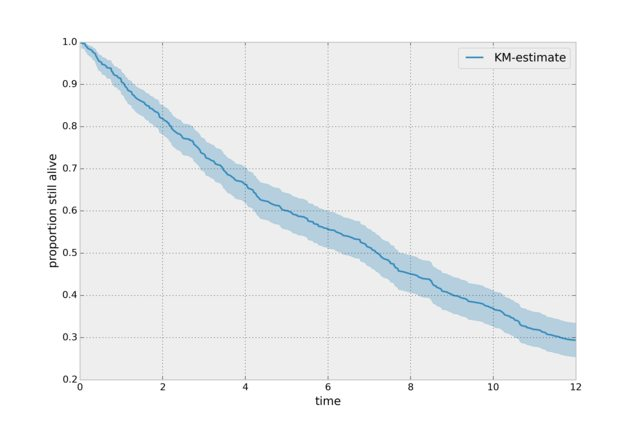
\includegraphics[width=0.9\linewidth]{lifelines-kmplot}
			\caption{}
			\label{fig:lifelines-kmplot}
		\end{figure}
		
	\end{frame}
	
	%================================================%
	\begin{frame}
		\begin{figure}
			\centering
			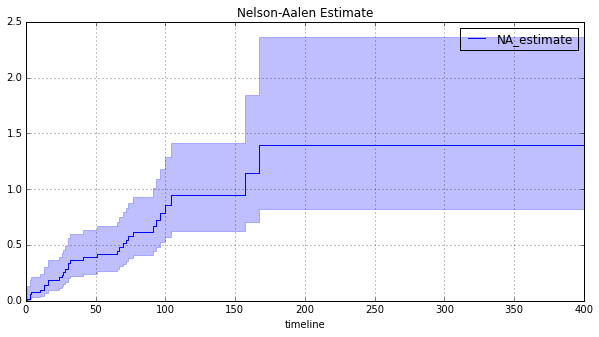
\includegraphics[width=0.9\linewidth]{lifelines-plotly-NAFplot}
			\caption{}
			\label{fig:lifelines-plotly-NAFplot}
		\end{figure}
		
	\end{frame}
	%=================================%
	\section{Cox Proportional Hazards Modelling}
	\begin{frame}
		\frametitle{Survival Analysis}
		\noindent \textbf{Cox Proportional Hazards Modelling}
		\begin{itemize}
			\item The Cox PH model gives a semi-parametric method of estimating the hazard function $\lambda$ at time $t$ given a baseline hazard that's modified by a set of covariates:
			
			%	λ(t|X)=λ0(t)exp(β1X1+⋯+βpXp)=λ0(t)exp(βX)
			
			\item where $\lambda_0(t)$ is the non-parametric baseline hazard function and $\beta_X$ is a linear parametric model using features of the individuals, transformed by an exponential function.
			
			\item The algorithm runs quite quickly, performing iterative partial regression of the time-dependent $\lambda_0(t)$, and the feature-dependent $exp(\beta_X)$, repeated until convergence.
		\end{itemize}
		
		
	\end{frame}
	%=================================%
	\begin{frame}
		\frametitle{Survival Analysis}
		The big strength of Cox PH is to:
		\begin{itemize}
			\item allow us to compare the relative hazard rates of the different features by comparing the $\beta$ coefficients, and to
			compute a predicted survival function for new datapoints simply by plugging the details into the model.
			\item 	One big weakness of the Cox PH is that the $\beta$ values are assumed constant over all time, which is often untrue, more of which later.
			
		\end{itemize}
		
		Lets continue our investigation into the harddrive failure data, and as ever, the plots and tables in the notebook are accompanied by detailed comments:
	\end{frame}
	%=================================%
	\begin{frame}
		\frametitle{Survival Analysis}
		
		To summarise the notebook:
		
		\textbf{Model specification}
		
		The first obvious difference we encounter with this regression method is to transform the row-based dataframe into a design matrix using the patsy package and a model-specification string manufacturer + capacity. 
		
		%This modelspec is simply a GLM1 and the flexible approach afforded by Cox PH lets us declare any modelspec we wish, for example rather than β0X0+β1X1+β2X2β0X0+β1X1+β2X2 we could try β0X20+β0X0+β1X1∗β2X2β0X02+β0X0+β1X1∗β2X2 etc.
		
	\end{frame}
	%=================================%
	\begin{frame}
		\frametitle{Survival Analysis}
		\noindent \textbf{Baseline hazard}
		
		\begin{itemize}
			\item The Cox PH model takes a few iterations to converge on a fit and the lifelines package stores several results on the \texttt{CoxPHFitter} object for convenience including the cumulative baseline hazard rate $\Lambda$ and baseline survival rate $S=e^{-\Lambda}$.
		\end{itemize}
		
		
	\end{frame}
	%=================================%
	\begin{frame}
		\frametitle{Survival Analysis}
		
		That baseline hazard rate increases to 1\% at approx 5 years power-on time. This has been set by whatever feature combination was set on the intercept, in this case manufacturer == HGST and capacity == 1.5TB which are quite low-failure values.
		
	\end{frame}
	%=================================%
	\begin{frame}
		\frametitle{Survival Analysis}
		
		Proportional Hazards
		\begin{itemize}
			\item The baseline is of course, modified by the relevant exp$(\beta X)$ values and it's here that we can make some interesting comparative observations on the model:
			
			\item An 'average' Seagate drive has approx 22x the hazard rate of an 'average' HGST drive, and approx 12x that of an 'average' WDC drive
			
		\end{itemize}
		
	\end{frame}
	%=================================%
	\begin{frame}
		\frametitle{Survival Analysis}
		\begin{itemize}
			\item A 'average' 3TB drive has a hazard rate approx 14x that of a 1.5TB drive and 3x that of a 4TB drive
			\item Combining features, our model tells us a Seagate 3TB drive has a hazard rate (22+14=36)(22+14=36)x that of the baseline; 2222x larger than an HGST 3TB drive, and 1010x larger than a WDC 3TB drive.
		\end{itemize}
	\end{frame}
	%=================================%
	\begin{frame}
		\frametitle{Survival Analysis}
		\begin{itemize}
			\item These ratios may seem surprising at first: can a Seagate 3TB drive really be an estimated 22x more likely to fail than an HGST 3TB drive? 
			\item Look back to the Kaplan-Meier modelling in the previous post and we see the survival functions for 3TB drive as measured by a Kaplan Meier model. 
			\item If we use the relation λ(t)=−log(S(t))and the comparison λ(t)Seagate.3TBλ(t)HGST.3TBλ(t)Seagate.3TBλ(t)HGST.3TB, we see:
		\end{itemize}	
		
		
	\end{frame}
	%=================================%
	\begin{frame}
		\frametitle{Survival Analysis}
		At 1 year, Seagate 3TB drives are log(0.987)log(0.997)=4.4log(0.987)log(0.997)=4.4x more likely to fail than HGST 3TB.
		At 2 years, log(0.85)log(0.994)=27log(0.85)log(0.994)=27x
		At 3 years, log(0.417)log(0.983)=51log(0.417)log(0.983)=51x
		... so the 22x multiplier is a reasonable value. This also neatly demonstrates a weakness of the Cox PH approach: the proportional hazards are modelled as time-invariant, whereas here we see a wide, time-varying range from 4x to 51x.
		
	\end{frame}
	\section{Model evaluation}
	%=================================%
	\begin{frame}
		\frametitle{Survival Analysis}
		Model evaluation
		\begin{itemize}
			\item We can use a concordance index and k-fold cross validation to evaluate the performance of the model, for more details see the Notebook itself.
			
			\item We find a mean average concordance of 0.76, which indicates a reasonably accurate model and we could quite happily use it to predict the survival of as-yet-unseen harddrives of the same manufacturers and capacities.
		\end{itemize}
		
		
	\end{frame}
	%=================================%
	\begin{frame}
		\frametitle{Survival Analysis}
		
		Weaknesses of the Cox PH model
		
		As shown above, we can't always assume that a comparative hazard rate is constant with time, for instance:
		
		time-to-first-purchase habits may initially differ greatly between shoppers who arrived at a website via different adverts, but those differences may disappear over time
		post-surgery, the probability curve of patient recovery differs between the young and the old over time
		in our harddrive data we see that 3TB Seagate drives have between 4x, 27x and 51x the hazard rate of HGST 3TB drives over the first 3 years of power-on
	\end{frame}
	%=================================%
	\begin{frame}
		\frametitle{Survival Analysis}
		Despite offering quick calculation and easily interpretable results, the central assumption of constant proportional hazards is a weakness of the Cox PH model. It's always useful to start a survival analysis with Kaplan-Meier and/or Cox PH in order to set a baseline, but we are unlikely to stop with these models and call it complete.
	\end{frame}
	%=================================%
	\begin{frame}
		\frametitle{Survival Analysis}
		Next steps
		For now, we'll pause this series here, since we've covered a lot of ground:
		\begin{itemize}
			\item In part 1 we described Survival Analysis as a method for measuring time-to-event behaviour and worked though several considerations including the hazard function, half-life and censoring
			\item In part 2 we demonstrated the preparation of an analysis environment using scientific Python, and also showed our acquiring, storing and preparing the harddrive failures data
			\item In part 3 we showed a set of initial analyses to further understand the data, and ran a few Kaplan-Meier models to discover the survival functions of the whole population and for specific drive manufacturers and capacities
		\end{itemize}
	\end{frame}
	%=================================%
	\begin{frame}
		\frametitle{Survival Analysis}
		And of course above, we've used a Cox PH model to describe the relative impact of different manufacturers \& capacities on harddrive failure rates, and we've also tested the model predictions using a standard concordance measure.
	\end{frame}
	\section{Other Modelling Approaches}
	%=================================%
	\begin{frame}
		When we return to this series we may discuss more complicated regression models which let us make more accurate and reasoned predictions, including:
	\end{frame}
	
	%=================================%
	\begin{frame}
		\frametitle{Survival Analysis}
		\noindent \textbf{Aalen Additive Model}
		
		This survival regression model extends the Cox PH concept to perform a piecewise linear regression on the cumulative hazard value at each point in time along the x-axis:
		
		%λ(ti)=∑j=1j=Nβ0(ti)+βj(ti)xj
		%λ(ti)=∑j=1j=Nβ0(ti)+βj(ti)xj
		where $\beta$j(ti) lets us have a time-varying covariate for feature $x_j$. We can also add normalisation parameters (e.g. L1 or L2 norms) to help smoothen the regressions.
	\end{frame}
	%=================================%
	\begin{frame}
		\frametitle{Survival Analysis}
		\noindent \textbf{Gaussian Process Regression}
		
		Gaussian Process models are a generic Bayesian method to estimating arbitrary functions using exogenous features. As a probabilistic method we gain great flexibility, data interpolation, empirical confidence intervals (credible regions) and the ability to include prior assumptions.
	\end{frame}
	%=================================%
\subsection*{Non Parametric Methods for Survival Analysis}
\begin{frame}
Nonparametric methods provide simple and quick looks at the survival experience, and the Cox proportional hazards regression model remains the dominant analysis method. 

%This seminar introduces procedures and outlines the coding needed in SAS to model survival data through both of these methods, as well as many techniques to evaluate and possibly improve the model. 

%Particular emphasis is given to proc lifetest for nonparametric estimation, and proc phreg for Cox regression and model evaluation.

Note: A number of sub-sections are titled Background. 
These provide some statistical background for survival analysis for the interested reader (and for the author of the seminar). 

Provided the reader has some background in surival analysis, these sections are not necessary to understand how to run survival analysis. 

These may be either removed or expanded in the future.

Note: The terms event and failure are used interchangeably in this seminar, as are time to event and failure time.
\end{frame}
%\subfile{Censoring.tex}
%\subfile{Nelson-Aalen.tex}
\end{document}